\tcbsection{What are the implications of the profile and progress data with respect to student performance since the prior self-study (or initial visit)?}

\minor{Notices from profile data since last self-study:}
\begin{itemize}
\item Increase in student population from 459 to 506
\item Developed a viable, actionable Campus Development Plan
\item Demographics have changed resulting in 3% increase in non-native English speakers
\item Assessments used previously are no longer valid as adopted standards have changed
\item In terms of tuition, the discount category has decreased while the standard category has increased thus providing more income for school growth.
\item Almost all CMIS graduates matriculate to postsecondary education. 
\item Schoolwide learner outcomes were updated to reflect measurability and global citizenship
\end{itemize}

\minor{Student Learner Outcomes}
Courageous Learners who: 
\begin{itemize}
\item Embody a work ethic that values learning and academic integrity
\item Pursue personal growth as adaptive, independent learners
\item Exhibit thinking that is open minded, creative, and takes risks
\item Utilize resources and technology to effectively support learning and work
\end{itemize}

Responsible Global Citizens who:
\begin{itemize}
\item Understand Christian virtues and positive student character 
\item Demonstrate integrity through consistent respect for people of all faiths
\item Develop cultural awareness and an appreciation for diversity
\item Serve as responsible, proactive members of the global community
\end{itemize}

Recognizing the need to instill citizenship and the CMIS core virtues, the school has taken steps to coordinate and promote our community values.  In the elementary program, our school counselor teaches weekly interactive virtues lessons to each grade level.  In addition the counselor, principal, teachers, and students facilitate a monthly Virtues Assembly that highlights a different virtue each month. These events are well attended by our community.

In order to instill a philosophy of giving to to those in need, the middle school students visit a local orphanage once each semester.  The students work with the volunteers and children by organizing activities and events to develop a sense community and global advocacy.  This fall, CMIS used the annual Harvest Festival as an opportunity to collect donated goods for Hope House, a local orphanage supported by members of the school community.  Every other Tuesday, middle school students pair with an elementary student to read a book aloud to them in the CMIS Reading Buddies program.  This enables our older students to serve as models to younger students.  

The entire school community has participated in the global initiatives, “Mix it up at Lunch Day” developed by Teaching Tolerance foundation and “Great Kindness Challenge”, organized by the Kids for Peace organization, to promote our school vision as place that respects and celebrates diversity. The “Mix it up at Lunch Day” encourages students to sit and interact with students that they may not know well. This is a simple act with profound implications. Studies have shown that interactions across group lines can help reduce cultural misunderstandings. When students interact with those who are different from them, biases and misperceptions can fall away.  The “Great Kindness Challenge”, encourages students to perform virtuous acts of kindness to students and adults on campus. In addition, middle school and high school students are assigned to communication groups, in which their teachers provide some level of individualized pastoral care.  

{\centering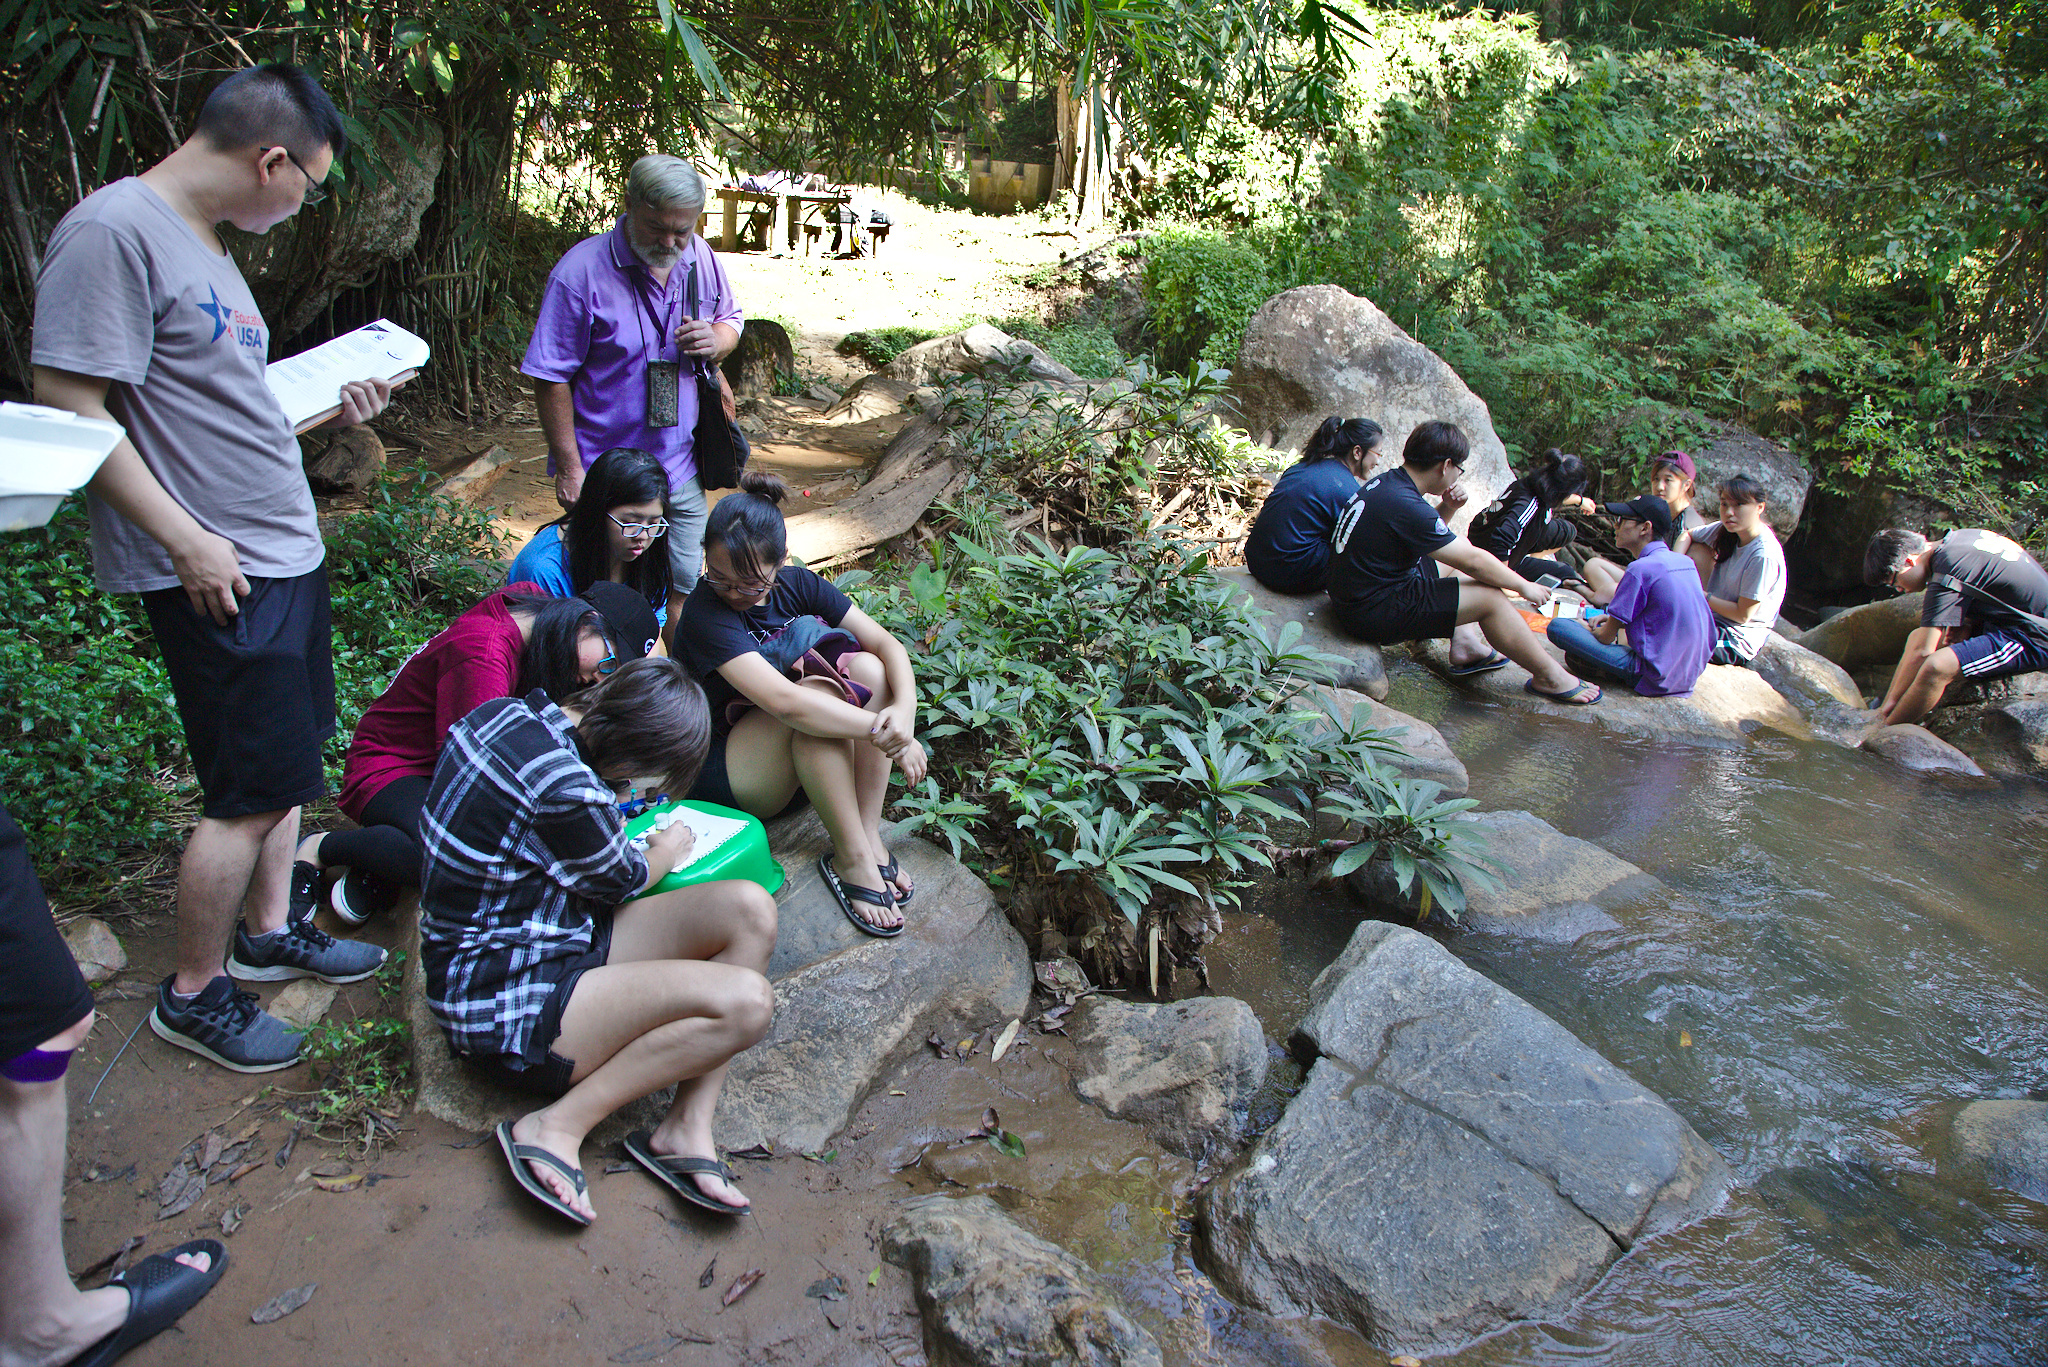
\includegraphics[width=\textwidth]{chapter3science_fieldtrip.jpg}}

High school students learn to take ownership of the schoolwide learner outcomes by participating in community service activities. The CMIS Community Service Coordinator has encouraged students to create their own community service projects that align with our schoolwide learner outcomes. This transfer of responsibility encourages student inspired community advocacy.  CMIS Leadership also encourages group community service projects that build student collaboration and group accountability. By earning community service credits, high school students demonstrate proactivity in planning and implementing their own projects.  Community service projects for high school students are also encouraged within the CMIS community, such as: 
\begin{itemize}
\item Reading Buddies to elementary students, which supports school cohesiveness (and student reading comprehension). 
\item Homework Club to middle and elementary students, which promotes student achievement in a caring environment. 
\item Parent facilitators, such as English translators, campus orientation guides, and childcare assistants during family conferences, which increases parent participation and develops student responsibility.
\end{itemize}

CMIS has sought to uphold the rich Christian heritage upon which it was founded while continuing to welcome those of differing religious backgrounds, cultures, and beliefs. Within this spirit, CMIS has encouraged students to learn about God’s love and the Christian faith so they can make their own personal and intelligent response to it. The all school Christmas and Easter assemblies, various prayer meetings, and weekly faith-based clubs have been designed with this purpose in mind. Each week, there are several different opportunities for students to be involved in learning more about the Christian faith if they desire. CMIS has a Student Spiritual Advisor to facilitate these faith based programs and to serve as a positive role model and advocate for all students.

CMIS has also modified the policies and procedures in the Student Planner/Handbook to emphasize research based best practices. Rather than focusing on repercussions of negative behaviors, the emphasis is on positive behaviors that create responsible and proactive members of the global community.  For example, addressing student digital citizenship, students practice how to respect intellectual property rights and to avoid plagiarism through engaging lessons and activities, rather than reviewing a list of consequences. 

Since the self-study, CMIS has taken steps to regularly analyze data. We adopted the Datawise process to help teachers through the process of analyzing student performance data. Teachers also regularly peer review assessments using a common peer review form. The CMIS Leadership has begun to create a culture of looking at data and will continue to use data to modify instruction in respect to student performance. CMIS Leadership Team also understands the need to create a online, data “sandbox” where we can access multiple forms data to help teachers analyze student performance and make instructional adjustments to address our learner needs.

CMIS has made significant improvements in both the resource adoption, request, and renewal process. Since CMIS adopted new standards in 2013, updated, aligned, rigorous, and engaging resources have been vetted, evaluated, and adopted in science and mathematics. All teachers are involved in the vetting, evaluation, and selection of adopted resources. All adoption meetings involved targeted professional development on the standards, rigor, and instructional shifts. 

In 2014-2015, CMIS began a development program to familiarize teachers with the CCSS Literacy standards and to create blueprints of unit studies and lesson plans using the Understanding by Design (UbD) approach. More time is required to fully implement these standards throughout their UbD units. Teachers worked in departments to create these blueprints and lesson plans with oversight from our Curriculum Director.  

\tcbsection{Based on past performance and current data, select two to three critical learner needs, noting the correlated schoolwide learner outcomes.}

Based on our reported percentage of students from an English-speaking background, CMIS is categorized differently by ISA each year. Thus, a year-by-year comparison with like schools is hard to make and interpret. Because of the challenge, the CMIS Teaching Staff have used the Datawise process since 2014, in which a study of the ISA data identified the need for students to further develop their expository/argumentative writing skills.  A school-wide writing assessment was given to further confirm this need, and an action plan was created to scaffold the students that needed extra attention with this particular skill. CMIS also used this opportunity to create a common assessment rubric for English Language Arts (ELA) and Social Studies departments. In 2015 the Datawise process indicated a need for student improvement in writing organization. Teachers researched and adopted department graphic organizers as a common intervention strategy. In 2016 the Datawise process indicated that student progress was difficult to evaluate as teachers within the same department were incorporating different assessment techniques and formats. It also highlighted the need for consistent, standards based, school-wide student data. As a result, teachers are currently working on the creation of consistent assessments and the school will be implementing the comprehensive assessment platform, Measure of Academic Progress (MAP), which is a standards-based assessment that can be implemented school-wide.

Based on the data we have found, while a majority of our students perform well on standardized tests (PSAT 8/9, SAT/NMSQT, SAT), some students are not reaching the College Board benchmarks. To correlate this with student performance in class, we need to provide teachers with timely PSAT data to determine the extent to which low PSAT performances are related to testing anxiety versus gaps in learning. Adding the MAP test will also add more data to help teachers identify skill deficits and modify instruction to meet student needs. Additionally, CMIS has included Grades 8 and 9 in PSAT testing in 2015-2016 to proactively address test anxiety and to give students an opportunity to practice SAT testing. 

\minor{Correlated SLOs}

Pursue personal growth as adaptive, independent learners, exhibit thinking that is open minded, creative, and takes risks, and utilizes resources and technology to effectively support learning and work.

\tcbsection{List 3-4 important questions that have been raised by the analysis of the student performance, demographic, and perception data and the progress data.  (These will be used in the Home and Focus Group work.)}

\minor{Question 1: How do our assessments align with the rigor of the standards?}

This question was given to teachers as they peer reviewed their assessments and evaluated student work samples. The purpose was to ensure that teachers were implementing the standards to the correct alignment and rigor as stated in the standard. This is a continuing discussion in department and divisional meetings.

\minor{Question 2: How did formative assessment inform one of your decisions today or this week with a student, a subset of students, or a class?}

This question was used to have teachers discuss the purpose of and the effective use of formative assessments in their classes. As formative assessment has played a central role in CMIS professional development for the past two years, CMIS Teaching staff have begun to reflect on this question with greater frequency. 

\minor{Question 3: How are we supporting students who have not demonstrated proficiency? }

This question was specifically used to analyze the way in which we identify struggling learners. It was also used to identify and remind teachers of the Student Support Team and how it is a resource for students’ academic, emotional, and social achievement.

\minor{Question 4: How can MAP and other standardized testing data be used to inform decisions?}

This question was used to overview the purpose of the MAP assessment. It encouraged teachers to identify the possible ways that large scale standardized testing can provide additional insight into their instruction. 

\minor{Question 5: How can we maintain our current student diversity in a growing international school market?}

This question was asked within the admission and leadership teams. It is an ongoing conversation that reflects upon the demographics of the Chiang Mai community and the increasing competition with local international schools. 
